\documentclass[letterpaper]{article}

\usepackage{natbib,alifeconf}  %% The order is important
\usepackage{url,hyperref,amsmath,cleveref}
\usepackage{booktabs}

% *****************
%  Requirements:
% *****************
%
% - All pages sized consistently at 8.5 x 11 inches (US letter size).
% - PDF length <= 8 pages for full papers, <=2 pages for extended
%    abstracts (not including citations).
% - Abstract length <= 250 words.
% - No visible crop marks.
% - Images at no greater than 300 dpi, scaled at 100%.
% - Embedded open type fonts only.
% - All layers flattened.
% - No attachments.
% - All desired links active in the files.

% Note that the PDF file must not exceed 5 MB if it is to be indexed
% by Google Scholar. Additional information about Google Scholar
% can be found here:
% http://www.google.com/intl/en/scholar/inclusion.html.


% If your system does not generate letter format documents by default,
% you can use the following workflow:
% latex example
% bibtex example
% latex example ; latex example
% dvips -o example.ps -t letterSize example.dvi
% ps2pdf example.ps example.pdf


% For pdflatex users:
% The alifeconf style file loads the "graphicx" package, and
% this may lead some users of pdflatex to experience problems.
% These can be fixed by editing the alifeconf.sty file to specify:
% \usepackage[pdftex]{graphicx}
%   instead of
% \usepackage{graphicx}.
% The PDF output generated by pdflatex should match the required
% specifications and obviously the dvips and ps2pdf steps become
% unnecessary.


% Note:  Some laser printers have a serious problem printing TeX
% output. The use of ps type I fonts should avoid this problem.


\title{Conchordal: Emergent Harmony via Direct Cognitive Coupling in a Psychoacoustic Landscape}


% Each submission will undergo a double-blind review process. To this end, submissions should NOT contain any element that could reveal the identity of the authors (author names, affiliations, funding details and acknowledgments), and should use the third person to refer to previous work by the authors.
\author{
    Koichi Takahashi$^{1}$$^{2}$
    \mbox{}\\
    $^1$Graduate School of Media and Governance, Keio University \\
    $^2$Conchordal.org \\
    info@conchordal.org
} % email of corresponding author

% For several authors from the same institution use the same number to
% refer to one address.
%
% If the names do not fit well on one line use
%         Author 1, Author 2 ... \\ {\Large\bf Author n} ...\\ ...
%
% If the title and author information do not fit in the area
% allocated, place \setlength\titlebox{<new height>} after the
% \documentclass line where <new height> is 2.25in

%% \newcommand{\optionalpaperfigure}[2]{%
%% \IfFileExists{#1}{%
%% \includegraphics[width=#2]{#1}%
%% }{%
%% \fbox{\parbox[c][0.22\textheight][c]{0.9\columnwidth}{\centering
%% Missing figure:\\\texttt{\detokenize{#1}}}}%
%% }%
%% }




% Choose one of: Full Paper, Summaries, or Late Breaking Abstracts 
% Submission type: \textbf{Full Paper}\\

% If sharing code / data, anonymize your repository and paste the link here.
% Example of anonymizing sevice for github: https://anonymous.4open.science/
% delete this line if not needed
% Data/Code available at: \url{http://your.repo.here.com}




\begin{document}

\maketitle

\begin{abstract}
This paper introduces \textit{Conchordal}, an artificial life system in which sonic agents inhabit and adapt within a psychoacoustic fitness landscape defined in log-frequency space. The environment integrates roughness (sensory dissonance) and harmonicity (periodicity-based virtual pitch coherence) into a continuous consonance field without presupposing musical scales or harmonic rules. Agents adjust pitch through local proposal-and-accept dynamics under density-based repulsion, regulate survival via a consonance-dependent metabolic policy, and entrain temporally through a Kuramoto-style phase coupling mechanism. Four empirical results are reported. (1) The psychoacoustic landscape exhibits attractors at simple frequency ratios. (2) Populations self-organize into structured, non-collapsed polyphony with enriched consonant interval distributions relative to ablated conditions. (3) When consonance modulates metabolic recharge, early consonance strongly predicts lifetime (Pearson $r \approx 0.71$; log-rank $p < 0.001$), whereas the effect vanishes without recharge. (4) External rhythmic coupling induces rapid phase locking (post-kick PLV $\approx 0.99$) across seeds. These findings demonstrate that consonance can function as an ecological resource in a non-traditional computational medium, yielding self-organization, selection, and synchronization in a unified sonic artificial life framework.
\end{abstract}

\section{Introduction}

Artificial life has traditionally unfolded in spatial, chemical, or symbolic domains \citep{langton1989,bedau2000}. Yet sound—despite its rich physical structure and deep entanglement with biological perception—remains largely unexplored as a primary computational medium for life-like dynamics \citep{miranda2002,eldridge2009}. Prior work has explored consonance-based harmony generation through navigation in perceptually motivated tonal spaces \citep{bernardes2016}; Conchordal instead treats consonance as an ecological resource within a continuous psychoacoustic field inhabited by autonomous agents. Conchordal advances a different premise: that psychoacoustic structure itself may constitute an ecological landscape in which adaptive agents evolve, interact, and synchronize.

Rather than encoding harmony or rhythm as compositional rules, Conchordal defines a continuous field derived from perceptual acoustics \citep{conchordal2025}. Agents do not “compose”; they seek locally advantageous regions of a cognitive landscape shaped by harmonicity and roughness. Consonance, in this system, is neither aesthetic nor normative; it is ecological. When linked to metabolism, it becomes a resource. When coupled to temporal oscillators, it enables entrainment.

The present study evaluates whether such a system satisfies core artificial life criteria: (i) self-organization under environmental constraints, (ii) selection mediated by resource dynamics, and (iii) synchronization through interaction and external forcing. Four experiments address these criteria.

\begin{figure*}[t]
\centering
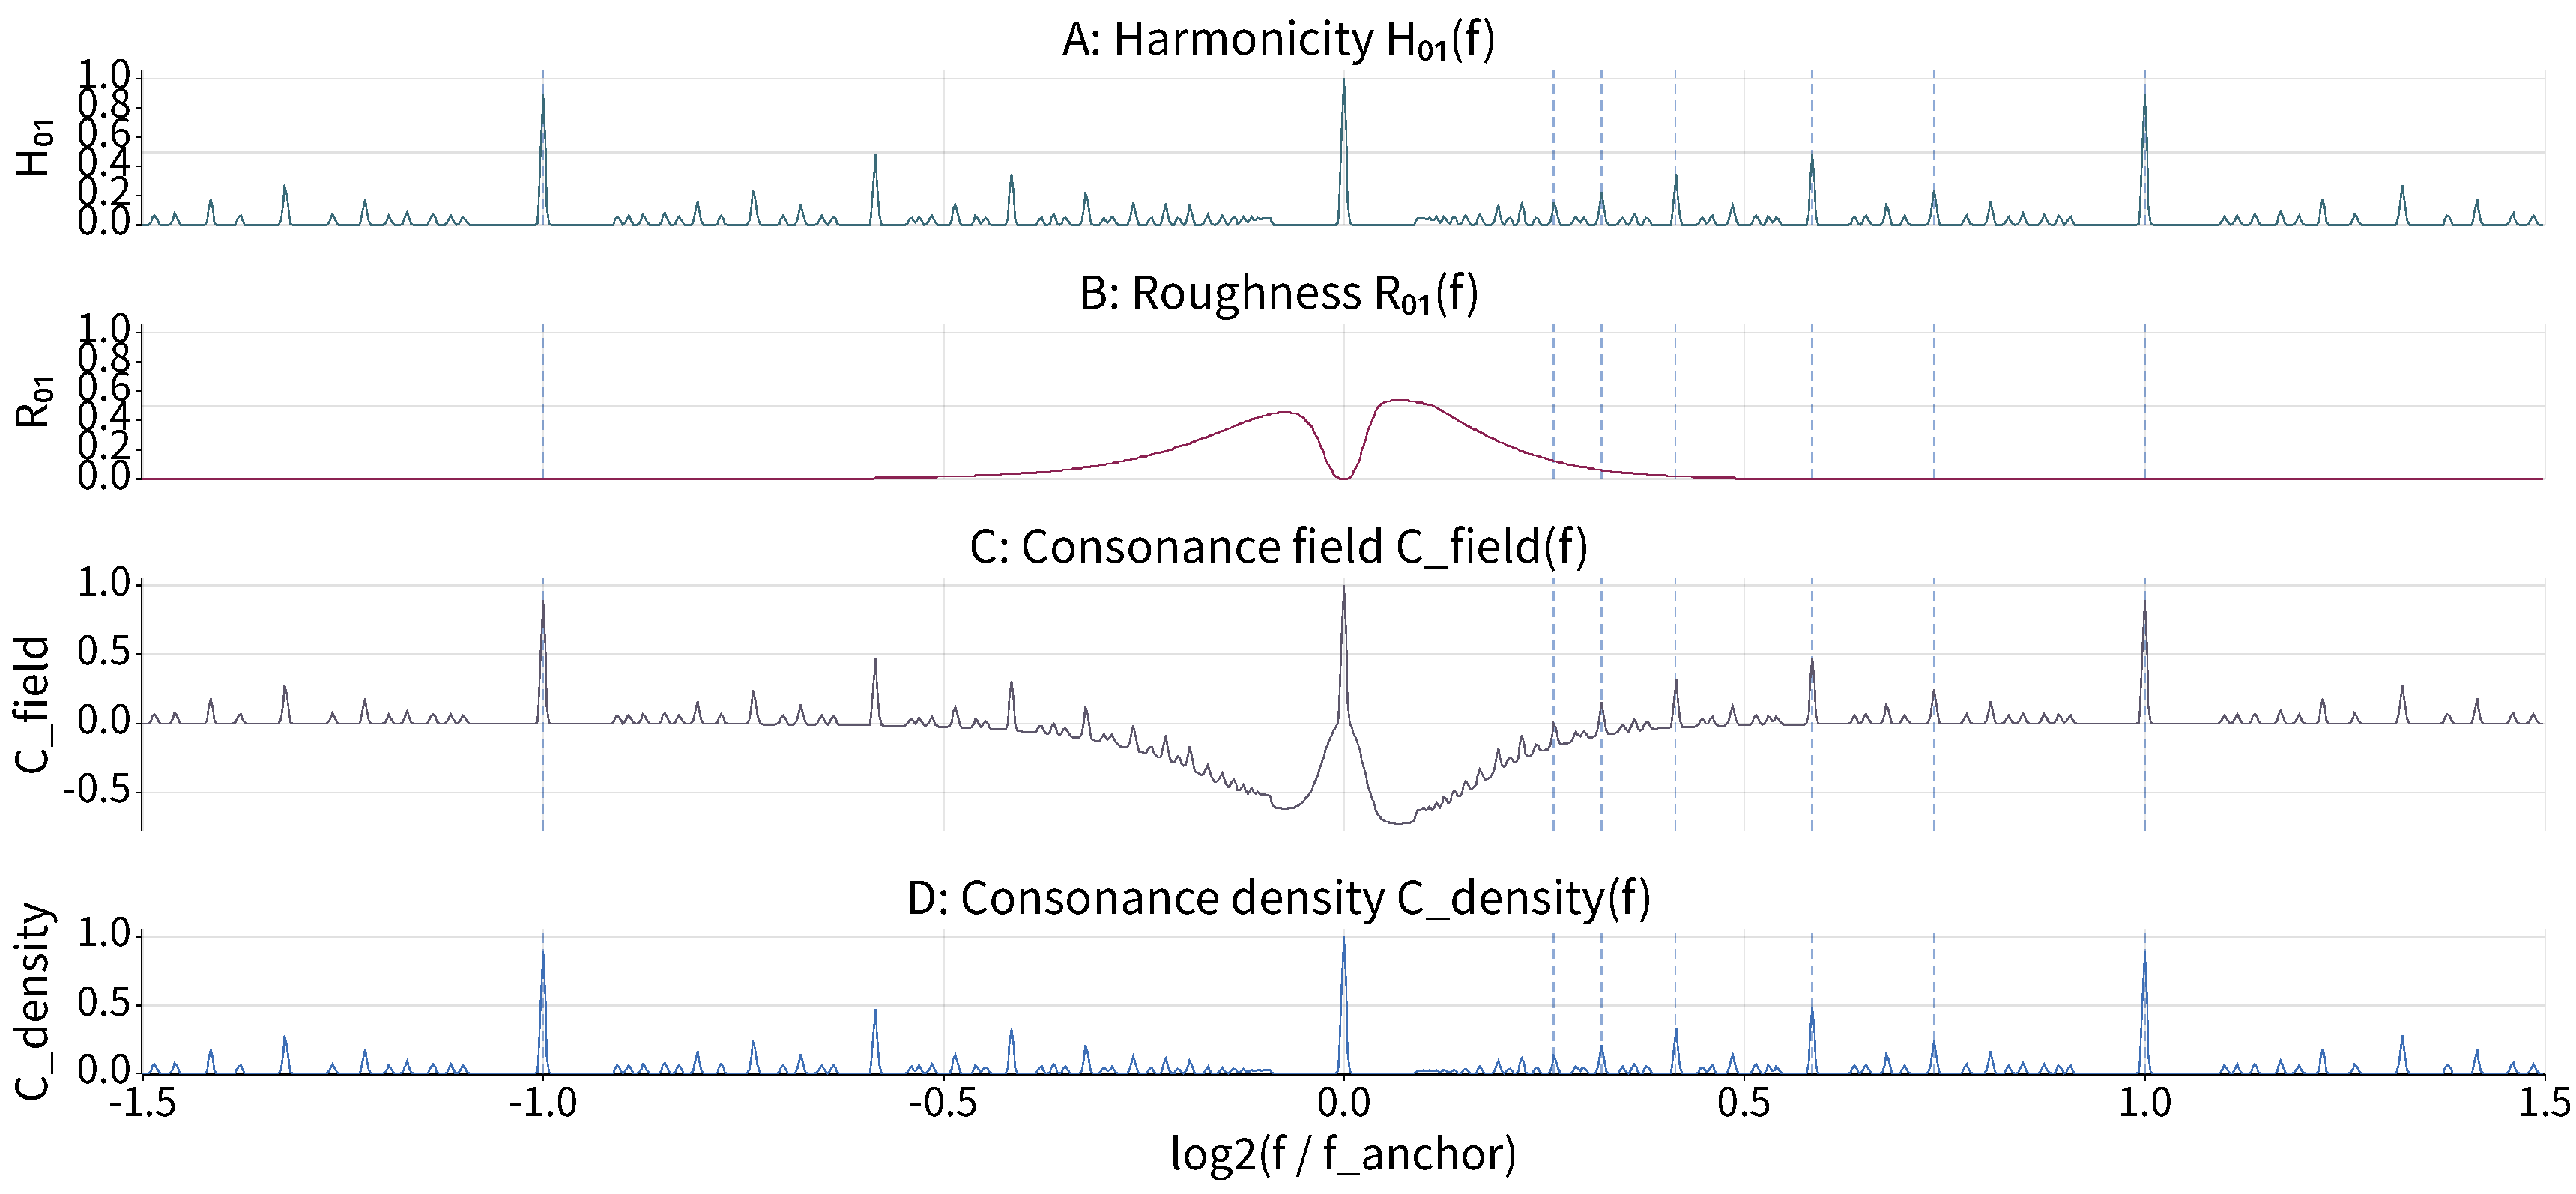
\includegraphics[width=\textwidth]{experiments/plots/e1/paper_e1_landscape_scan_anchor220.pdf}
\caption{Psychoacoustic landscape scan around an anchor tone (220\,Hz). (A)~Harmonicity $H_{01}(f)$; (B)~roughness $R_{01}(f)$; (C)~consonance field $C_{\text{field}}(f)$; (D)~consonance density $C_{\text{density}}(f)$. Vertical guides mark selected integer-ratio references relative to the anchor; the darker central line marks unison. Peaks at simple ratios in $H$ and corresponding troughs in $R$ combine to produce attractor structure in both consonance views. The reduced peak density outside $\pm 1$ octave is a finite-order sibling-projection property ($N=16$), not a plotting artifact.}
\label{fig:e1-landscape}
\end{figure*}

\section{The Psychoacoustic Landscape}

\subsection{Log-Frequency Representation}

All spectral relations are computed in log$_2$ frequency space. This coordinate system renders frequency ratios translationally invariant: intervals correspond to additive displacements. Such invariance is essential for modeling perceptual similarity structured by integer ratios rather than absolute frequency \citep{glasberg1990}.

Let $x = \log_2(f)$. Intervals become $\Delta x = \log_2(f_2/f_1)$. This representation allows harmonic templates and interference kernels to be defined as convolutional operations across a continuous domain.

\subsection{Harmonicity}

Harmonicity $H(x)$ quantifies how well spectral energy at position $x$ in log$_2$-frequency space is explained by a harmonic template \citep{terhardt1979,parncutt1988}. Periodicity extraction---the neural basis of virtual pitch---is well localized in the auditory brainstem and primary auditory cortex, making $H$ a relatively low-level, culture-invariant quantity.

Computation proceeds by sibling projection, a two-pass convolution with power-law weights $w_k=k^{-\rho}$ ($\rho>0$):
%
\begin{align}
  \mathrm{Roots}(x) &= \sum_{k=1}^{N} S(x+\log_2 k)\;k^{-\rho},
      \label{eq:h-down}\\
  H(x) &= \sum_{m=1}^{N} \mathrm{Roots}(x-\log_2 m)\;m^{-\rho}.
      \label{eq:h-up}
\end{align}
%
The downward pass (\ref{eq:h-down}) accumulates evidence for virtual roots; the upward pass (\ref{eq:h-up}) redistributes that evidence to harmonics. For two tones at frequency ratio $p\!:\!q$, coincident harmonics accumulate constructively; the number of such coincidences within order $N$ grows as $\max(p,q)$ shrinks, so peaks at simpler integer ratios are systematically stronger (Figure~\ref{fig:e1-landscape}A).

In all experiments $N=16$ and $\rho=0.4$. Overtone and undertone projections are blended with equal weight; full parameterization is given in \citet{conchordal2025}. The field is normalized to $H_{01}\in[0,1]$.

\subsection{Roughness}

Roughness $R(x)$ quantifies sensory dissonance from unresolved beating within the critical band \citep{plomp1965}. Like harmonicity, roughness reflects early peripheral processing: it arises from amplitude-modulation products on the basilar membrane, a mechanism rooted in cochlear mechanics \citep{glasberg1990}.

The computation maps the amplitude spectrum $S$ onto the ERB-rate scale $z = 21.4\log_{10}(0.00437f+1)$ and convolves with a Plomp--Levelt interference kernel:
%
\begin{equation}
  R_{\mathrm{raw}}(z) = \int S(\zeta)\;g_{\mathrm{PL}}(|z-\zeta|)
      \,d\zeta,
  \label{eq:roughness}
\end{equation}
%
where $g_{\mathrm{PL}}$ peaks at approximately $0.25$\,ERB and vanishes at both zero separation (no self-interference) and wide separation (outside the critical band). At simple integer ratios $p\!:\!q$, harmonics are spaced well beyond the critical band, producing roughness troughs that complement the harmonicity peaks (Figure~\ref{fig:e1-landscape}B).

The raw output is normalized via a reference-based saturation map to $R_{01}\in[0,1]$; details are given in \citet{conchordal2025}.

\subsection{Consonance}

Unlike harmonicity and roughness, which each correspond to a well-localized stage of auditory processing, consonance is not a single well-defined perceptual quantity. Its evaluation recruits higher-order circuits---from cortical pitch maps through prefrontal valuation networks---and is further shaped by enculturation and listening context. No unique mapping $C(H,R)$ can therefore be stipulated on purely psychoacoustic grounds.

In Conchordal, consonance serves multiple computational roles: landscape evaluation for hill-climbing pitch adaptation, bounded metabolic signaling, and nonnegative mass for density-weighted proposal sampling. We address both the definitional indeterminacy and this diversity of downstream uses by adopting a bilinear consonance core---the most general first-order interaction model for two $[0,1]$ inputs:
%
\begin{equation}
C = a\,H_{01} + b\,R_{01} + c\,H_{01}\,R_{01} + d.
\label{eq:consonance-core}
\end{equation}
%
Here $b<0$ penalizes roughness, while $c>0$ weakens that penalty when harmonicity is high. Different coefficient settings yield task-specific quantities from the same functional family.

The evaluation field for local pitch adaptation uses $(a,b,c,d)=(1,-1.35,1,0)$:
\begin{equation}
C_{\text{field}} = H_{01} - 1.35\,R_{01} + H_{01}\,R_{01}.
\end{equation}

For density-based proposal weighting, we set $(a,b,c,d)=(1,0,-\rho,0)$ with $\rho=1$, yielding a dedicated nonnegative mass:
\begin{equation}
C_{\text{density}} = H_{01}(1 - R_{01}).
\end{equation}

This separation avoids conflating acceptance utility ($C_{\text{field}}$) with proposal density ($C_{\text{density}}$). Figure~\ref{fig:e1-landscape}C,D illustrates the resulting landscape for a single-anchor scan; both views exhibit attractor structure at simple integer ratios.

For bounded metabolic control, $C_{\text{field}}$ is passed through a sigmoid:
\begin{equation}
C_{\text{level01}} = \sigma\!\bigl(\beta(C_{\text{field}}-\theta)\bigr)\in[0,1], \quad (\beta,\theta)=(2,0).
\end{equation}

\section{Agents and Dynamics}

\subsection{Pitch Adaptation}

Each agent proposes local pitch perturbations sampled within a bounded neighborhood in log-frequency space. A hill-climbing acceptance rule evaluates candidate positions via consonance and a density-based repulsion term. Repulsion is computed through a Gaussian kernel over pitch distances, discouraging collapse to identical frequencies.

Ablation conditions remove either the hill-climbing mechanism or the repulsion term.

\subsection{Metabolic Policy}

Agents possess energy $E$. Dynamics follow:

\begin{equation}
E' = E - c_b \Delta t - c_a I_{\text{attack}} + r \cdot C_{\text{level01}} \cdot I_{\text{attack}},
\end{equation}

where $c_b$ is basal cost, $c_a$ attack cost, and $r$ recharge coefficient. In the baseline condition, recharge scales with consonance; in the ablation condition, recharge is set to zero. Agents perish when $E$ falls below threshold.

\subsection{Temporal Oscillation}

Each agent contains a phase oscillator:

\begin{equation}
\dot{\phi_i} = \omega_i + \frac{K}{N}\sum_j \sin(\phi_j - \phi_i) + F(t).
\end{equation}

Here $K$ is coupling strength and $F(t)$ is an optional external forcing term (“kick”). Phase locking is quantified via the Kuramoto order parameter $r(t)$ \citep{kuramoto1984,strogatz2000} and phase-locking value (PLV) \citep{lachaux1999}.

\section{Results}

\subsection{Landscape Attractors}

As shown in Figure~\ref{fig:e1-landscape}, scanning a single anchor frequency across log-frequency space confirms that harmonicity peaks at simple integer ratios (2:1, 3:2, 4:3, 5:4), while roughness exhibits corresponding troughs \citep{helmholtz1877,sethares1993}. Both $C_{\text{field}}$ and $C_{\text{density}}$ exhibit attractor structure near small-integer ratios. No discrete scale was imposed; the attractors emerge solely from psychoacoustic structure.

\subsection{Self-Organized Polyphony}

Populations of 24 agents were simulated for 100 steps (burn-in 10). Three conditions were compared: baseline, no hill-climb, and no repulsion.

\begin{figure*}[t]
\centering
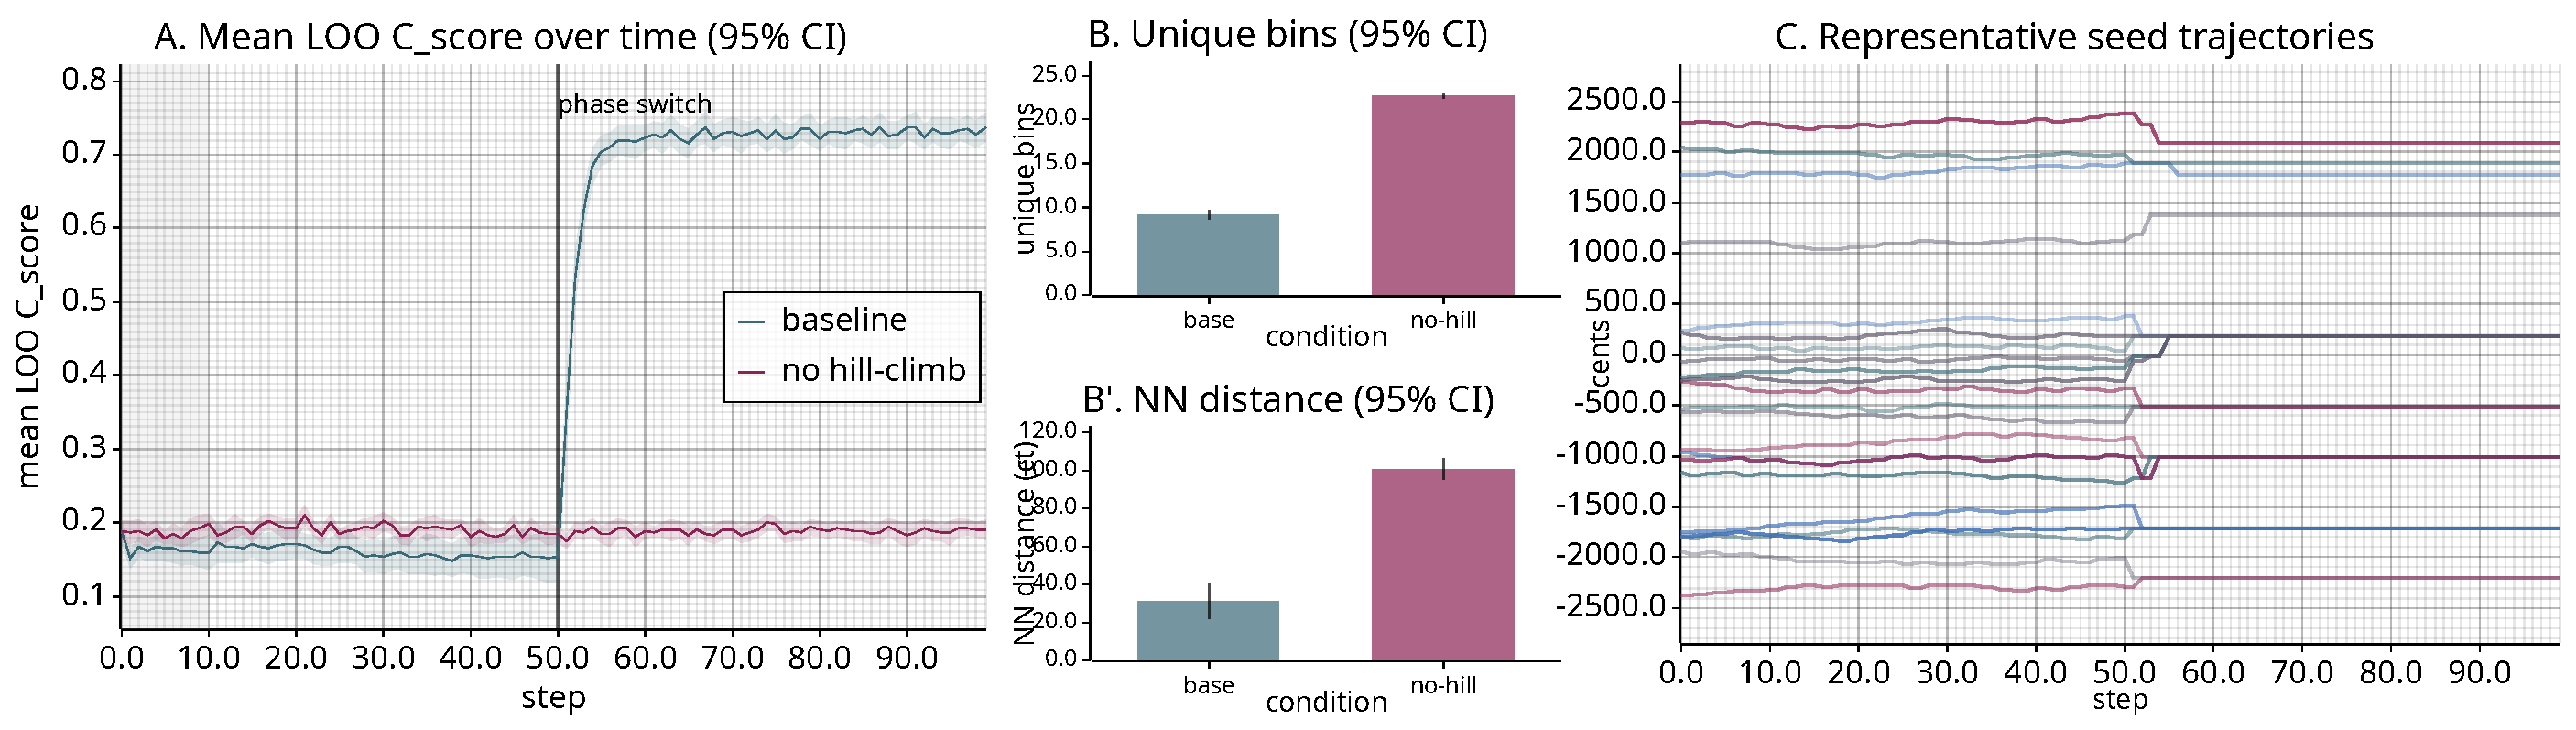
\includegraphics[width=\textwidth]{experiments/plots/e2/paper_e2_figure_e2_1.pdf}
\caption{Population dynamics and diversity. (A) Mean consonance over time (95\% CI); the vertical marker indicates the programmed phase switch. (B) Unique pitch bins at end of run (95\% CI). (B') Mean nearest-neighbor distance (st, 95\% CI), revealing pronounced collapse when repulsion is removed. (C) Representative seed trajectories in semitone units.}
\label{fig:e2-dynamics}
\end{figure*}

\textbf{Diversity.} Unique pitch bins averaged 20.0 (baseline) versus 13.4 (no repulsion). Nearest-neighbor distances halved under no-repulsion, indicating collapse.

\textbf{Interval Structure.} The mass of consonant intervals \{3,4,7 semitones\} was 0.1596 in baseline, reduced to 0.1384 without hill-climbing. Entropy increased under no-hill (less structure) and decreased under no-repulsion (degenerate concentration).

These results show that hill-climbing enriches consonant interval structure, while repulsion prevents monophonic collapse \citep{reynolds1987}. Self-organized harmonic distributions arise from the landscape–agent interaction.

\begin{figure*}[t]
\centering
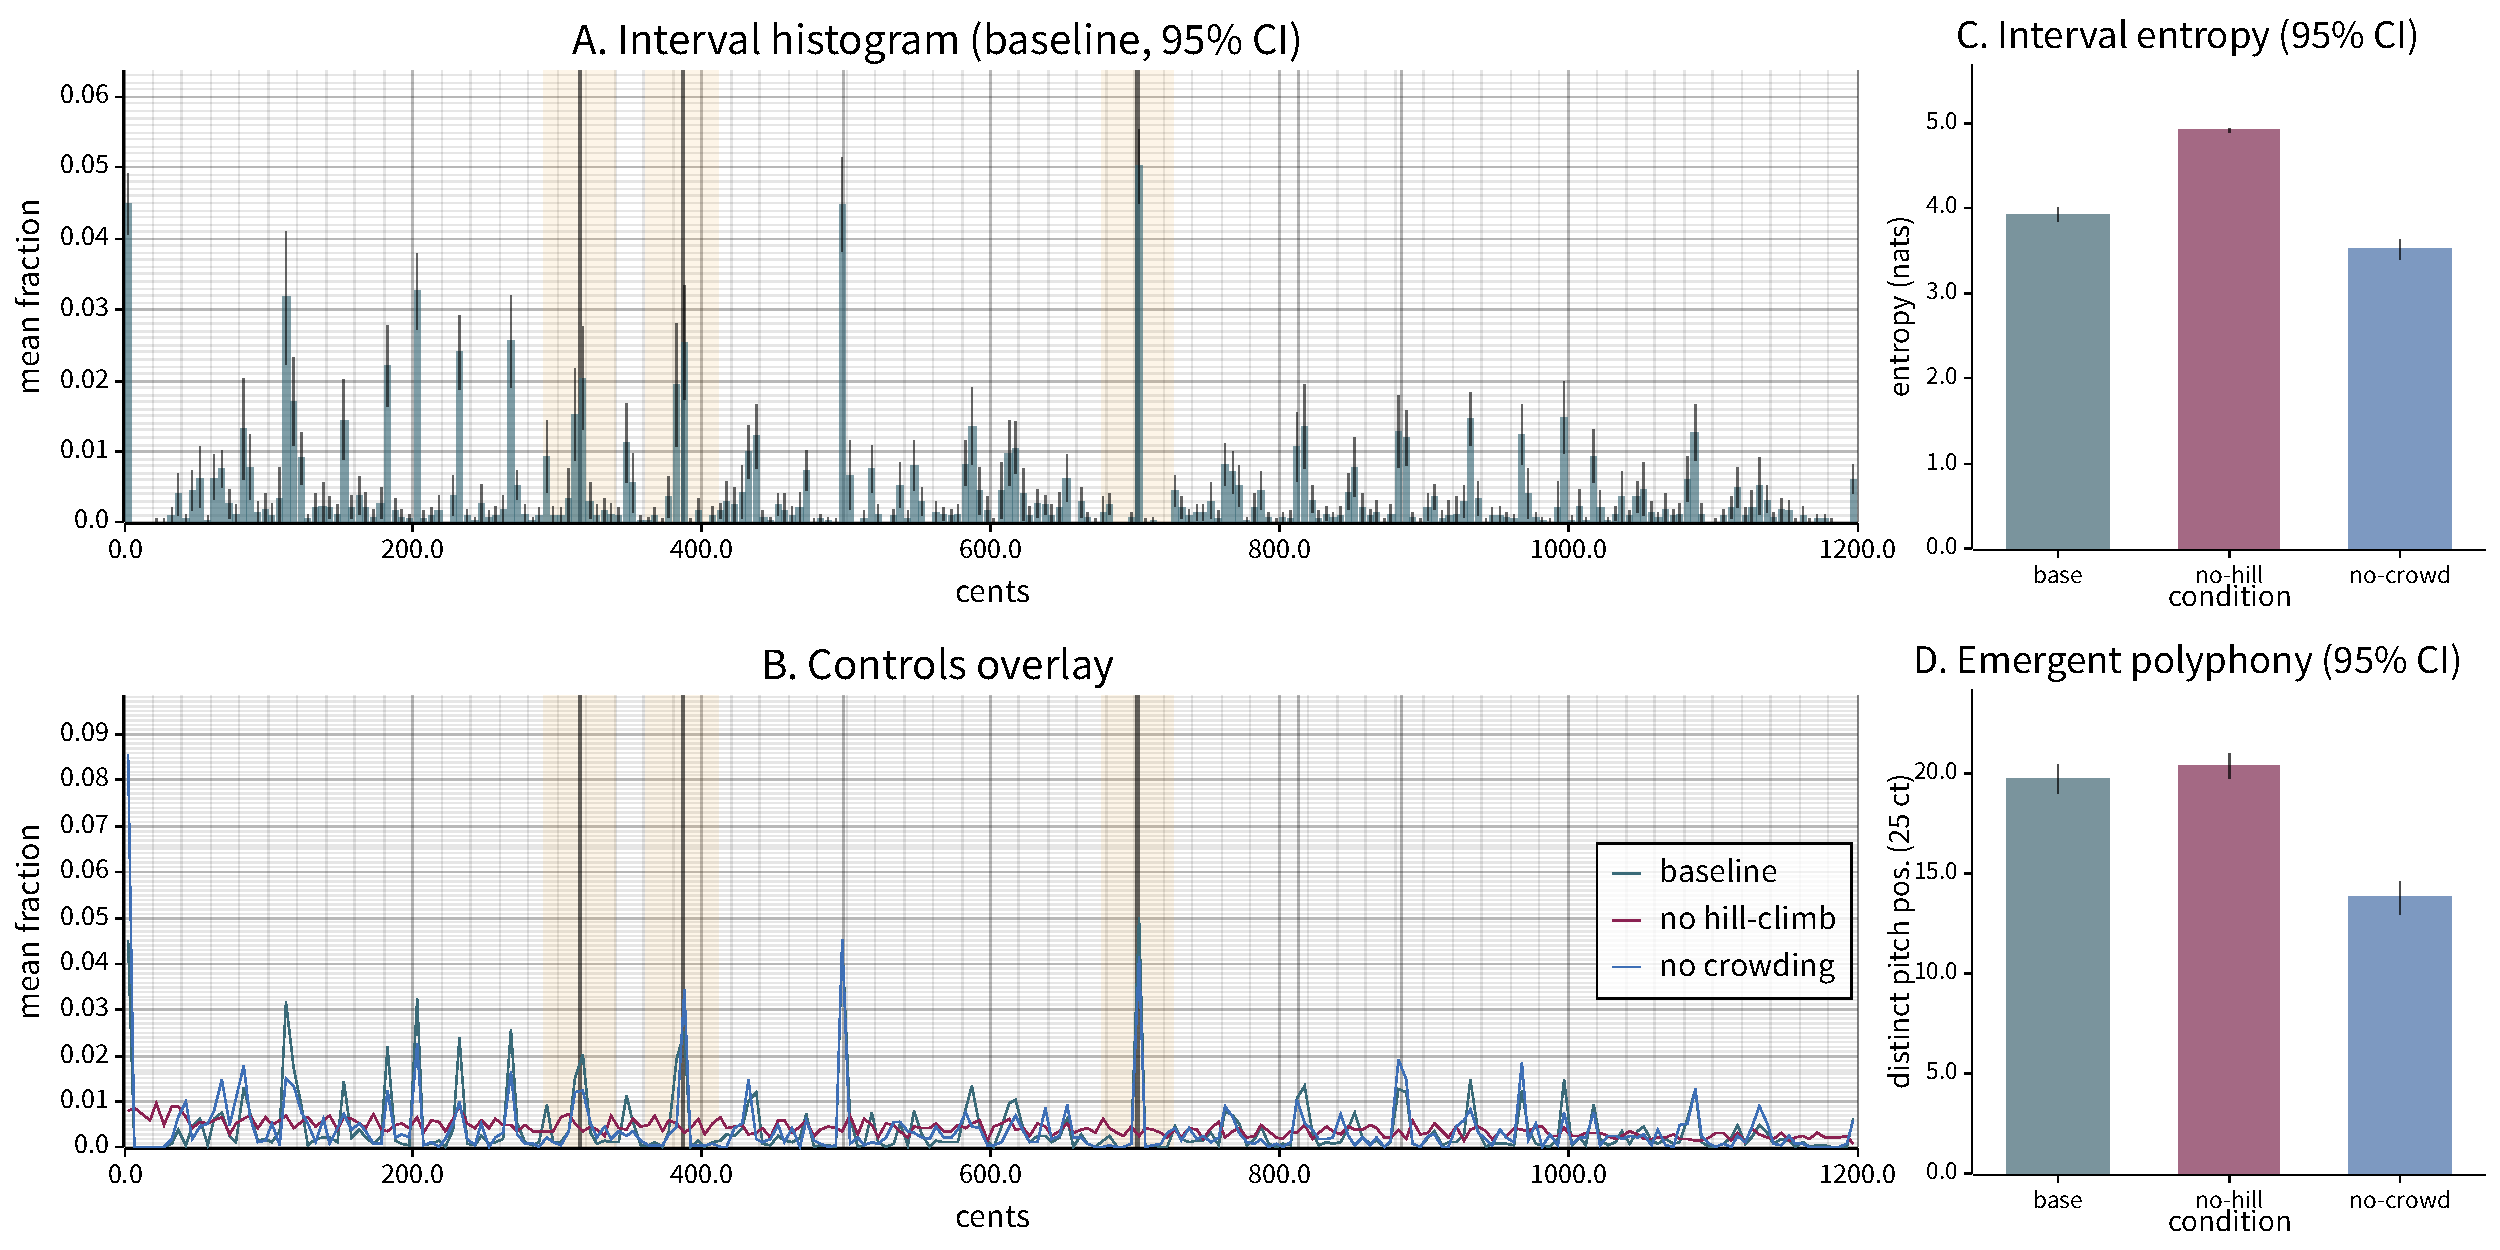
\includegraphics[width=\textwidth]{experiments/plots/e2/paper_e2_figure_e2_2.pdf}
\caption{Emergent interval structure and consonant mass. (A) Pairwise interval histogram for the baseline condition (mean with 95\% CI). (B) Overlay of baseline and ablations, displaying how hill-climbing and repulsion redistribute interval mass. (C) Consonant interval mass (95\% CI) for $T=\{3,4,7\}$ semitones. (C') Expanded set $T=\{0,3,4,5,7,8,9\}$. Hill-climbing systematically enriches consonant mass; removing repulsion destabilizes the distribution.}
\label{fig:e2-intervals}
\end{figure*}

\subsection{Consonance as Selection Pressure}

Across 1000 pooled runs, early consonance (first 20 ticks) strongly predicted lifetime under baseline recharge (Pearson $r = 0.7096$; Spearman $\rho = 0.4513$; log-rank $p < 0.001$). Median survival differed markedly between high- and low-consonance groups (372 vs. 339).

When recharge was disabled, correlations vanished (Pearson $r = 0.028$; log-rank $p = 0.33$). Thus, consonance functions as a genuine ecological resource, generating measurable selection pressure.

\begin{figure}[t]
\centering
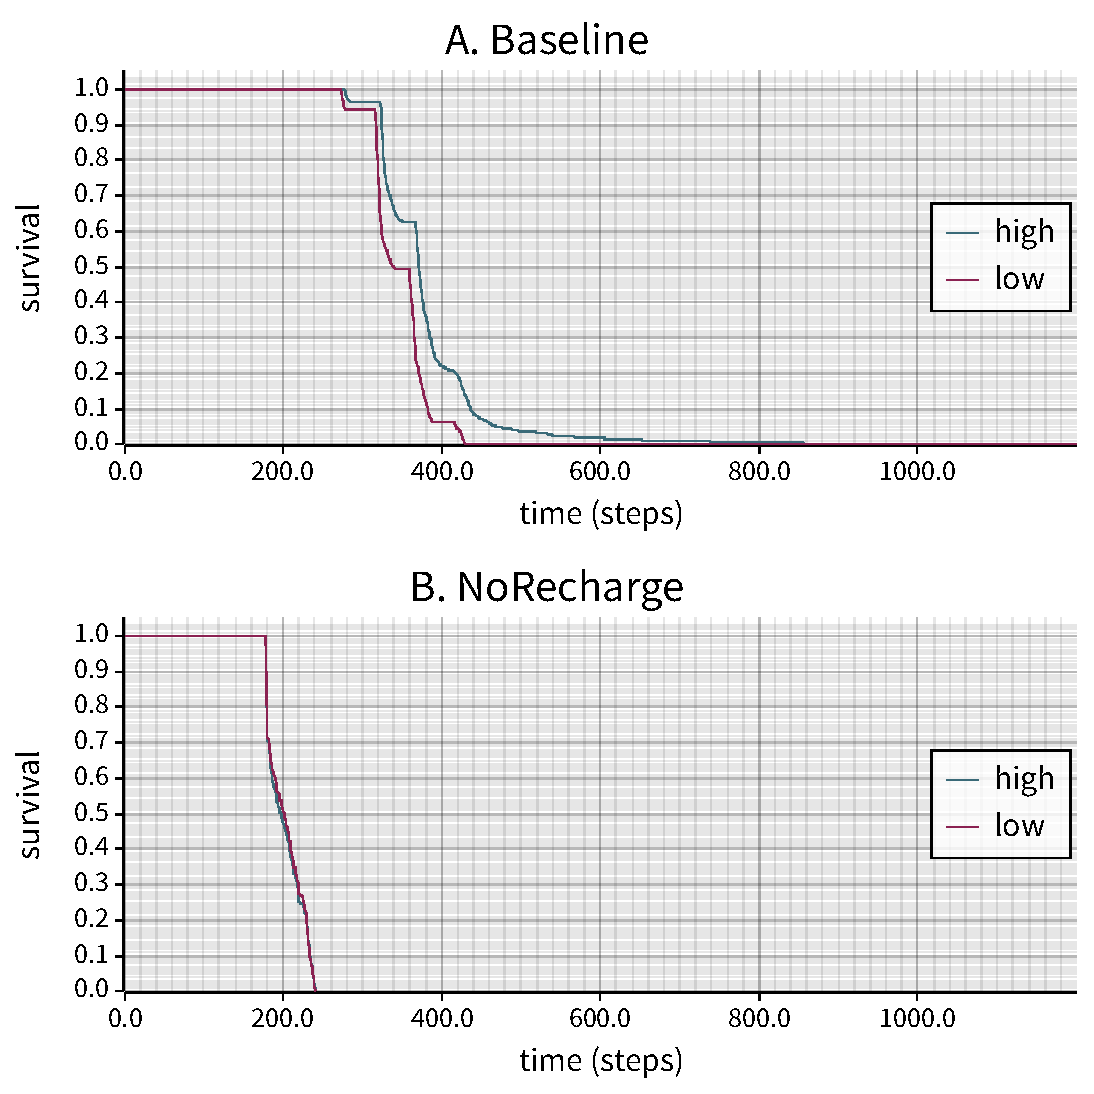
\includegraphics[width=\columnwidth]{experiments/plots/e3/paper_e3_firstk_survival_compare_pooled.pdf}
\caption{Consonance-dependent metabolism induces selection. Kaplan--Meier survival curves for agents split by early consonance (median split of $C_{\mathrm{level01,firstK}}$, pooled; $n_{\mathrm{high}}=500$, $n_{\mathrm{low}}=500$). Left: baseline recharge yields a pronounced survival advantage for high-consonance agents (median 372 vs.\ 339 steps; log-rank $p<0.001$). Right: removing recharge eliminates the effect (median 199 vs.\ 197; log-rank $p=0.330$).}
\label{fig:e3-selection}
\end{figure}

\subsection{Rhythmic Entrainment}

Simulations over 40 seconds introduced an external forcing (``kick'') at 16 seconds. Before forcing, main and control conditions overlapped (PLV $\approx 0.225$). After forcing, the main condition rapidly converged to PLV $\approx 0.993$ ($\pm 0.021$), while control remained near baseline ($\approx 0.226$).

The order parameter \citep{kuramoto1984} approached unity only in the coupled condition. Synchronization therefore emerges from dynamical interaction rather than spontaneous drift.

\begin{figure*}[t]
\centering
\includegraphics[width=0.49\textwidth]{experiments/plots/e5/paper_e5_order_over_time.pdf}\hfill
\includegraphics[width=0.49\textwidth]{experiments/plots/e5/paper_e5_plv_over_time.pdf}

\medskip
\includegraphics[width=0.35\textwidth]{experiments/plots/e5/paper_e5_seed_sweep.pdf}
\caption{Rhythmic entrainment under external forcing (“kick”). Top-left: Kuramoto order parameter $r(t)$ for main and control conditions; pre-kick overlap reflects $k_{\mathrm{eff}}=0$, while the kick rapidly drives the main condition toward near-unity coherence. Top-right: phase-locking value (PLV) to the kick; the main condition converges to PLV $\approx 1$ whereas the control remains near baseline. Bottom: seed sweep summary of post-kick PLV mean, demonstrating robustness across runs. Vertical markers indicate burn-in end, kick onset, and evaluation start.}
\label{fig:e5-entrainment}
\end{figure*}

\section{Discussion}

Conchordal demonstrates that psychoacoustic structure can support artificial life phenomena without recourse to symbolic encoding or predefined tonal systems. Three properties are notable.

First, consonance is not imposed but computed from physical and perceptual principles \citep{helmholtz1877,plomp1965}. The landscape attractors (Figure~\ref{fig:e1-landscape}) reflect integer-ratio periodicity inherent to harmonic spectra \citep{terhardt1979}.

Second, harmonic structure in populations arises from local optimization and density constraints. No global coordination or compositional rule is required.

Third, when consonance modulates energy, ecological selection appears \citep{bedau2000} (Figure~\ref{fig:e3-selection}). Agents that occupy more consonant regions survive longer. Removing recharge abolishes the effect, confirming causality.

Finally, temporal synchronization (Figure~\ref{fig:e5-entrainment}) shows that rhythmic coherence can be induced through oscillator coupling, linking pitch ecology and temporal order within one framework.

Collectively, these findings position sound as a viable non-traditional medium for artificial life, satisfying criteria of self-organization, selection, and synchronization.

\section{Limitations and Future Work}

The present system lacks reproduction and mutation; evolutionary dynamics remain indirect. Future work may incorporate lineage-based adaptation and open-ended spectral diversification. Additionally, perceptual models could be extended to include inharmonic spectra or timbral dimensions.

Empirical validation with human listeners would further test whether emergent structures align with perceived harmonic organization.

\section{Conclusion}

Conchordal establishes a psychoacoustic artificial life environment in which consonance acts as an ecological resource. In log-frequency space, harmonicity and roughness define a continuous landscape supporting attractors, population-level structure, survival differentials, and rhythmic entrainment. These results suggest that life-like adaptive dynamics need not be confined to spatial or chemical substrates. Sound itself—structured by perceptual law—can sustain artificial ecologies.

\bigskip

\noindent\textbf{Keywords:} Artificial Life, Psychoacoustics, Consonance, Self-Organization, Synchronization, Computational Music Systems

\bibliographystyle{apalike}
\bibliography{conc}

\end{document}
